\section{Mô tả thiết kế kiến trúc để xây dựng hệ thống}
    \quad Sau khi xác định rõ bài toàn, dựa trên những yêu cầu cả về mặt chứng năng và phi chức năng, nhóm quyết định đưa ra thiết kế hệ thống như sau:

    \vspace{1cm}
    \begin{figure}[h]
    	\centering
    	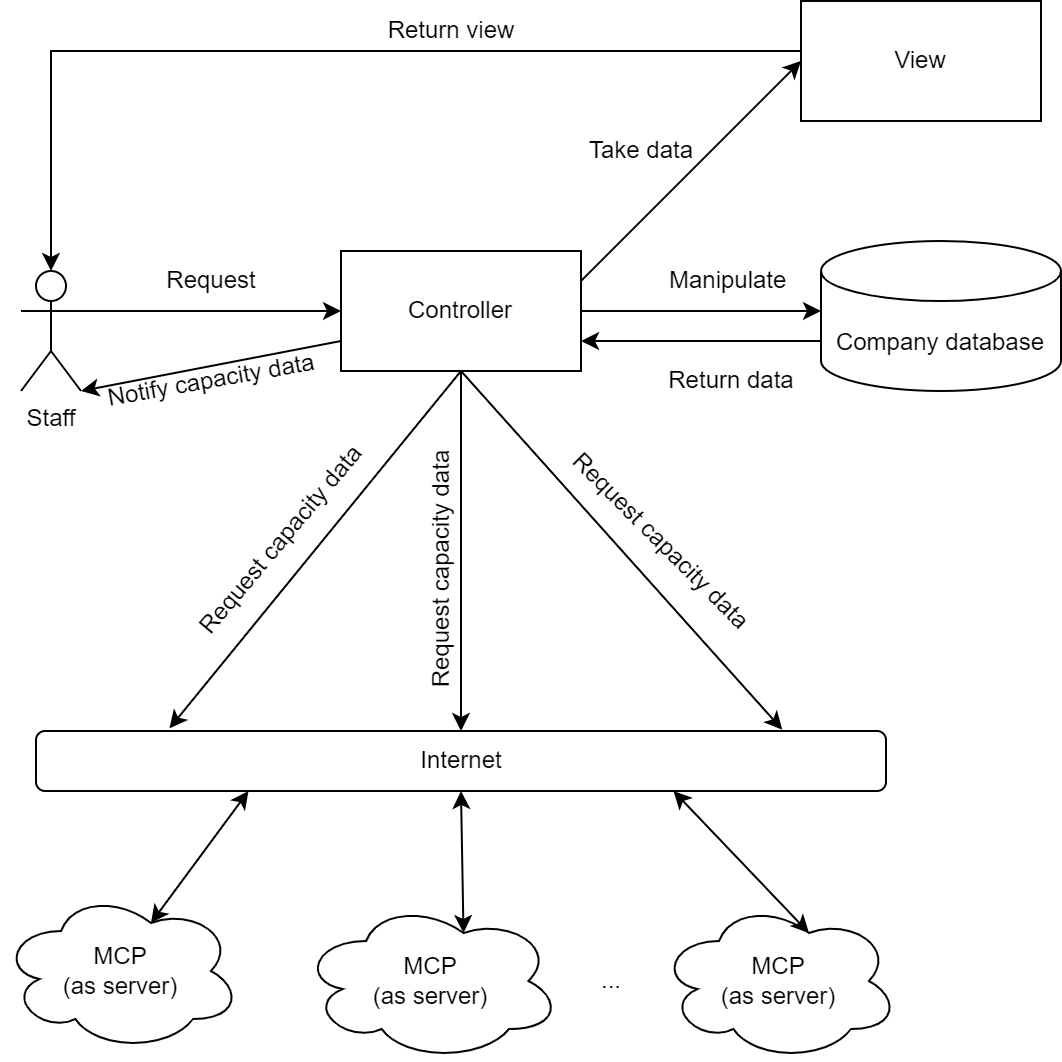
\includegraphics[width=1\linewidth]{imgs/architecture design.png}
    	\caption{Thiết kế kiến trúc của hệ thống}
    \end{figure}

   	\begin{tblr}{
   			width=1\linewidth,
   			hlines,
   			vlines,
   			colspec={X[3]X[7]},
   			columns = {valign = m, },
			column{1} = {halign = c},
   			row{1} = {halign = c, valign = m, bg = lightgray, fg = black},
   		}
   		{\textbf{Table} & \textbf{Architecture design}}  \\
   		Pattern		& 	MVC + Pub-sub \\
   		Description & 	1. Với các thông tin cơ bản như thông tin cá nhân, lịch làm, thông tin về phương tiện, ta sử dụng mô hình MVC để lấy dữ liệu và hiển thị lên cho người dùng. \newline
						\newline
		   				2. Với các thông tin về sức chứa của các MCP, ta sử dụng mô hình publisher - subscriber với Controller đóng vai trò là subscriber và MCP là các publisher. \newline
						\newline
		   				3. Với các thông báo về việc sức chứa của các MCP đạt mức tối đa ta sử dụng mô hình publisher - subscriber với Controller lúc này đóng vai trò là publisher và nhân viên là các subscriber. \\
		Flow & 			1. Controller nhận request từ người dùng -> gọi đến database thực hiện yêu cầu -> database gửi kết qua sau khi thực hiện lại cho controller -> controller gửi dữ liệu vừa nhận được cho phần View -> View hiển thị kết quả cho người dùng. \newline
						\newline
						2. Controller nhận dữ liệu từ tất cả các sensor của từng MCP sau mỗi 15 phút. Nếu sau ba lần controller không nhận được dữ liệu, sensor xem như bị mất kết nối và thực hiện thiết lập lại kết nối với sensor của MCP đó. \newline
						\newline
						3. Ngay sau khi nhận dữ liệu từ các sensor, controller thực hiện broadcast dữ liệu nếu sức chứa đã đầy đến collector/janitor liên quan đến MCP đó. \\
   	\end{tblr}

   	\vspace{0.5cm}

	\quad \textbf{Những nguyên nhân nhóm chọn kiến trúc trên:}
	\begin{enumerate}
		\item[-] MCP (Model - Controller - View) là kiểu kiến trúc bao gồm 3 chủ thể lớn là Controller - đảm nhiệm việc kiểm tra và thực hiện các yêu cầu được gửi đến, Model - đảm nhiệm việc truy suất dữ liệu của hệ thống và View - là cái được trả về cho người dùng, cái được hiển thị trên màn hình. MCP phù hợp với yêu cầu hiện thực ứng dụng trên nền tảng web, dễ dàng trong việc thiết kế, triển khai hệ thống.
		\item[-] Publisher - Subcriber cho cho phép hệ thống nhận thông tin liên tục về các điểm MCP và gửi đến người dùng những thông tin kịp thời nhất khi một hay nhiều điểm MCP bị đầy.
		\item[-] Xét tương đối với các kiến trúc khác:
		\begin{enumerate}
			\item[+] Mặc dù Layer và MCV đều được thiết kế theo kiểu module, trong đó các khối được tách ra đảm nhiệm từng chức năng riêng biệt, khi cần nâng cấp một module sẽ không ảnh hưởng đến hoạt động của các module khác. Tuy nhiên MVC có hiệu suất tốt hơn Layer, vì dữ liệu được truyền qua một tầng duy nhất, khác với việc khi truyền dữ liệu ở kiến trúc Layer phải đi qua nhiều lớp dẫn tới hao phí thời gian truyển dữ liệu từ lớp này sang lớp kia
			\item[+] Peer-to-Peer là kiểu thiết kế trong đó các client sẽ kết nối trực tiếp với nhau, trong trường hợp ứng dụng quản lý có số lượng lớn các client (bao gồm back officer, janitor, collect), việc kết nối trực tiếp các thiết bị sẽ gây ra sự chồng chéo, khó khăn trong việc kiểm soát cũng như bảo trì
			\item[+] Pipe-filter có lợi thế trong	 việc tách dữ liệu có độ phức tạp cao thành dữ liệu sạch thông qua các lớp màn lọc (filter), tuy nhiên hạn chế của kién trúc này là ở việc với những nguồn data khác nhau, nó sẽ yêu cầu một luồng riêng, khả năng tái sử dụng các luồng cũ rất thấp. Đối với bài toán mà nhóm đang giải quyết, việc dữ liệu mà các MCP trả về là khác nhau, nguyên nhân có thể do sự khác biệt về phần cứng hay phần mềm của các cảm biến, chính vì thế nếu sử dụng Pipe-filter thì ta phải tạo ra nhiều luồng xử lý đối với từng MCP.
		\end{enumerate}
	\end{enumerate}
  
	\newpage
   	\quad Đối với bài toán được đặt ra, ta sẽ có tổng cộng 6 module. Bao gồm:
   	\begin{enumerate}
   		\item Module Xác thực

   		\begin{tblr}{
   				width=1\linewidth,
   				hlines,
   				vlines,
   				colspec={X[3]X[7]},
   				columns = {valign = m, },
   			}
   			Input & Người dùng X \\
   			Output & Người dùng X có được truy cập hay không \newline
   					 Vai trò của người dùng X là gì \\
   			Method & Validation() \newline
   			 		 Login() \newline
   			 		 Logout() \newline
   			 		 ChangePassword() \\
   		\end{tblr}

   		\item Module Chat

  		\begin{tblr}{
  				width=1\linewidth,
  				hlines,
  				vlines,
  				colspec={X[3]X[7]},
  				columns = {valign = m, },
  			}
  			Input & Tin nhắn, văn bản\\
  			Output & Hệ thống gửi tin nhắn cho người dùng \newline
  					 Người dùng nhận được tin nhắn \\
  			Method & ConnectUser() \newline
		  			 SendMessage() \newline
		  			 NotifyMessage() \\
  		\end{tblr}

  		\item Module View information

  		\begin{tblr}{
  				width=1\linewidth,
  				hlines,
  				vlines,
  				colspec={X[3]X[7]},
  				columns = {valign = m, },
  			}
  			Input & MCP X \newline
  			Phương tiện Y \newline
  			Nhân viên Z \\
  			Output & Thông tin của MCP X \newline
  			Thông tin phương tiện Y \newline
  			Thông tin nhân viên và lịch làm của nhân viên Z \\
  			Method & ShowInfoMCP() \newline
  			ShowInfoVehicle() \newline
  			ShowInfoStaff() \newline
  			ShowDailyTask() \newline
  			ShowCalendar() \\
  		\end{tblr}
   		

   		\item Module Manage Resource

   		\begin{tblr}{
   				width=1\linewidth,
   				hlines,
   				vlines,
   				colspec={X[3]X[7]},
   				columns = {valign = m, },
   			}
   			Input & Nhân viên X, phương tiện Y\\
   			Output & Nhân viên X được chỉnh sửa \newline
   					 Phương tiện Y được chỉnh sửa \\
   			Method & AddUser() \newline
		   		     EditUser() \newline
		   			 DeactivateUser() \newline
   					 \newline
		   			 AddVehicle() \newline
		   			 EditVehicle() \newline
		   			 DeactivateVehicle() \\
   		\end{tblr}
   		
		\newpage
   		\item Module Planning route

   		\begin{tblr}{
   				width=1\linewidth,
   				hlines,
   				vlines,
   				colspec={X[3]X[7]},
   				columns = {valign = m, },
   			}
   			Input & MCP, Vehicle \\
   			Output & Tuyến đường khả dụng \\
   			Method & GenerateRoute() \newline
	   				 PlanRoute() \newline
	   				 GetAvailablePaths() \newline
	   				 ModifyRoute() \newline
	   				 ValidateRoute() \newline
	   				 GetPathsBetween() \newline
	   				 ValidatePath() \\
   		\end{tblr}

   		\item Module Task assign

   		\begin{tblr}{
   				width=1\linewidth,
   				hlines,
   				vlines,
   				colspec={X[3]X[7]},
   				columns = {valign = m, },
   			}
   			Input &	Nhân viên X \newline
   				    Công việc Y \\
   			Output & Công việc được chia thành công cho nhân viên \newline
   					 Thông báo lịch làm cho nhân viên \\
   			Method & CreateTask() \newline
   					 SetMCP() \newline
   					 SetVehicle() \newline
   					 SetSchedule() \newline
   					 AssignTask() \\
   		\end{tblr}

   	\end{enumerate}
\newpage
